\documentclass[type=dr, dr=rernat, accentcolor=tud7b,colorbacktitle, bigchapter, openright, twoside, 12pt ]{tudthesis}
\usepackage[english]{babel} 
\usepackage[utf8]{inputenc}
\usepackage{graphicx}
\usepackage{pstricks}
\usepackage{psfrag}
\usepackage{enumerate}
\usepackage{float}
\usepackage{epsfig}
%\usepackage{geometry}
\usepackage{subfigure}
\usepackage{rotating}
\usepackage{minitoc}
\usepackage{appendix}

\usepackage{tikz}

%%%% 1 1/2 facher Zeilenabstand:	
\usepackage{setspace}
\onehalfspacing


\begin{document}

\dominitoc
% in big toc display only chapters and sections
\setcounter{tocdepth}{1}
\tableofcontents

\chapter{Discussion}
\minitoc

The treatment planning results presented in the previous chapters are the first feasibility study to investigate the use of carbon ions 
for a non-invasive treatment of atrial fibrillation (AF). Cardiac target volumes like the pulmonary veins (PVs) or the atrioventricular (AV) node 
move due to respiration of the patient as well as due to heartbeat motion. When treating moving targets with a scanned carbon ion beam 
interference effects between the particle delivery and the interfractional target motion are observed, leading to over and under dosages in 
the target volume. This so-called interplay effect endangers the treatment outcome. Motion mitigation techniques are hence needed in order to diminish the influence of 
the motion. For respiration a gated irradiation around the end-exhale phase of the patients was studied. For heartbeat motion rescanning was 
studied. Thereby an averaging of different interplay patterns into a homogeneous dose is applied. The findings of treatment planning studies 
with motion mitigation techniques are discussed in section \ref{diss:mmt} of this chapter. 
The underlying motion size and motion direction will be discussed beforehand in section \ref{diss:motion}. 
% While the respiration is a motion 
% with a large amplitude, causing the PVs to move of up to 2cm, the heartbeat motion has a small amplitude and leads to a PVs and AV motion of 
% less than 7mm. 
Moreover, as the target volumes are surrounded by critical structures and organs at risk (OAR) like esophagus, trachea and 
aorta a close analysis of the OAR dose depostion was carried out. The findings will be discussed in section \ref{Dose:OAR} and the 
reduced dose deposition in comparison to a non-invasive treatment with photons will be shown in section \ref{Dose:OAR:photons}. 


\newpage

\section{Dose deposition}

In the here presented feasibility study of a non-invasive treatment of AF with carbon ions, a physical dose of 25Gy was 
applied in all treatment plans. This dose was chosen according to the publication by Sharma et al. \cite{Sha10}  
in which it was stated as the minimal needed dose in order to see an electrophysiological effect induced by photon irradiation. 
% % induce an electrophysiological change in the conduction system of the heart with a photon beam. 
% The planned studies in animal models with a carbon ions will show if higher or lower doses are in fact needed for this radiation type 
% and if biological effects need to be considered or can be neglected for such a high dose. 
% % Also closer analysis of biological effects of carbon ions and the hence resulting RBE might differ from the preliminary results of a negligable RBE. 
Older studies with photons in animal models support the finding by Sharma et al. in which doses higher than 20Gy seem 
to be sufficient in order to induce fibrotic tissue. A short overview will be given in section \ref{Dose:Target}.\newline
\newline
A close analysis of the dose deposition to the OARs was carried out in the here presented work, both for human data (chapter XXX) and the 
thereby studied PVs ablation, as well as for porcine data (chapter XXX) when irradiating the AV node. 
The findings will be discussed in section \ref{Dose:OAR} and a comparison with photon irradiation will be given in \ref{Dose:OAR:photons}. 
For critical structures like the aorta, esophagus, trachea and the heart itself dose-volume limits from SBRT were used \cite{RTOG0631} \cite{RTOG0915}. 
As the heart is not only an OAR in this studied treatment, but the target site itself, the dose-volume limits for this organ were often 
exceeded. Closer analysis of the irradiated cardiac substructures was hence performed.  



\subsection{Dose to target area}
\label{Dose:Target}

% - OUTLOOK: escalation study in pigs will show 
% - Greco mit 24 Gy
% - OUTLOOK: biodosis scheint vernachlaessigbar

In the paper by Sharma et al.\cite{Sha10} they stated that a dose of at least 25Gy is needed in order to induce an change in the 
conduction system of the heart with photon beams. Nevertheless also higher doses have been applied in the animal model study, 
reaching up to 80Gy. Part of the planned animal experiments at GSI will be a dose escalation study, in which the needed carbon ion dose for the 
generation of the desired fibrosis in the target area will be closer examined. It is already known from former studies on the 
effect of radiation on the heart which dose depositions as single fraction doses are sufficient in order to induce fibrotic tissue.\newline
\newline
Fajardo et al. \cite{Faj70} \cite{Faj73} investigated the evolution of radiation induced myocardial damage after a single dose 
of 20Gy in rabbits as well as a fractionated treatment, both with 6MV photons. They stated that their findings were independent of the 
time course of the irradiation, hence if the dose was applied as a single fraction or in different fractions. They found that there are three 
distinct stages in the evolution of radiation induced cardiac damage and divided it into an acute phase (an inflammtion within the first 
48hours), a latent stage (which can last up to seventy days) and the late stage where fibrotic lesions occur. Their explanation for the formation of fibrotic 
tissue is a failure of microcirculation, resulting from a failure of the complete reconstruction of capillaries in the endothelial cells after 
irradiation. They state that the occuring ischemia leads to myocardium fibrosis, which becomes maximal beyond 120 days.\newline
\newline
Other studies by Phillips et al. \cite{Phi64} and Bishop \cite{Bis65} et al. irradiated hearts of dogs and rodents with single photon doses 
of 60Gy to 96Gy. Both authors stated that they found severe functional abnormalities as well as myocardial 
fibrosis or even necrosis \cite{Ste68}. Efskind et al. \cite{Efs56} found fatal myocardial damage after 80Gy photon irradiation to the heart 
of rabbits.\newline
\newline
It can thus be assumed that the required dose for the desired generation of fibrotic tissue in the cardiac target volumes 
will require at least 20Gy, while high single fraction doses of up to 60Gy might induce necrosis, which needs to be avoided. 


\subsection{Dose to OAR}
\label{Dose:OAR}
In the studied human data it was found that the dose deposition in the aorta and trachea were uncritical and did not exceed the 
stated dose-volume limits. This was valid for all the studied safety margins (3mm, 5mm and 7mm) of the target volume, independent of the fact 
that the OAR dose deposition correlates with margin size.
The esophagus on the other hand is an endangered organ due to its proximity to the studied irriation site of the 
PVs. Different beam directions and field channel numbers were studied, none which resulted in a satisfactory sparing of this structure. 
Dose-volume exceeding results were already obtained for a small safety margin of 3mm in some patient cases, or even without the usage of 
any margin in other cases. An IMRT treatment was hence necessary, where the maximal dose to the esophagus was implemented in the dose 
optimization process. Thereby two different IMRT settings were used. One which was planned to deposit not more than a maximal dose of 17.5Gy 
(70\% of 25Gy) in this organ and one with a maximal dose of 7.5Gy (30\% of 25Gy) to the structure. While the weaker restriction already led to 
an improved result, the dose depositions were still too high, for one patient case even with only 3mm margin. The stronger restriction on the 
other hand resulted in dose depositions that did not exceed the dose-volume limit in all studied patient cases and for all studied safety margins. 
The IMRT restrictions for the esophagus even led to a further reduced dose deposition in the trachea of the studied patients due to the 
direct proximity of these two organs in respect of the used beam channel directions. 
In order to guarantee a safe delivery in a potential patient application a dedicated protocol to secure the esophagus of a too high dose 
deposition is nevertheless needed. Possible solutions to detect range uncertainties before the delivery of the high single fraction dose 
are stated in \ref{ceCT}. Analog to studies by Rucinski et al. \cite{Ruc13}, Christodouleas et al. \cite{Chr13} and van Gysen et al. \cite{Gys14} for prostate cancer 
or studies by Viswanathan et al. \cite{Vis13} for gynecologic cancers it could furthermore be studied if the 
injection of a spacer like hydrogel would be beneficial in order to increase the distance between the esophagus and the ablation sites. 
% % Analog to studies by e.g. el Bentefour et al. \cite{Ben12}, where in vivo range verifications were 
% % successfully achieved with a small dose deposition (<0.5cGy) in silicone diodes, a possible solution could be to predeposit the resulting 
% % treatment plan with a small dose in the order of mGy. By placing such an detector with a heart cather inside the patient, either in front of 
% % or inside the esophagus, this would allow to test for range of the planned energies and hence test for potential miscalculation or 
% % interfractional changes of the organs. 
Even though the dose-volume limits for the heart were exceeded, it should be noted that the heart is also the target volume in this 
feasibility studied. Further analysis of the maximal point dose, the maximal irradiated volume as well as the median 
dose were in good agreement to limitations stated in literature \cite{Gag10} \cite{Mar98} \cite{Wei08} \cite{Han93} and hence no pericarditis 
should be expected. Concerning the irradiated cardiac substructures it was found that three beam directions yielded a lower mean dose 
to the LCA. A mean dose over all patient cases of up to 1.5Gy for 7mm safety margin was found. According to a study by Darby et al. \cite{Dar13} 
major coronary events increase by 7.4\% per Gy photon irradiation after five years post radiotherapy. Due to the advanced age of the 
atrial fibrillation patient cohort the irradiation of the coronary arteries might hence play a less significant role.\newline 
\newline
Due to the anatomical differences of pigs compared to humans and due to the larger distance of the AV node to critical structures (esophagus, 
trachea and aorta) dose depositions to OAR for the irradiation of the AV node in the planned animal model were found to be negligible. 
Dose-colume limits were not exceeded and the stated OARs as well as the radiosensitive cardiac substructures were well spared. 
The dose-volume limits for the heart were also not exceeded. Maximal point dose to the heart as well as maximal irradiated volume and 
mean dose were also in very good agreement to the literature findings for human data. Late effects due to e.g. coronary events would 
also not be expected from the obtained dose deposition in this structures and are moreover irrelavant due to the short lifespan of the 
animals used in the planned animal model feasibility study planned at GSI.
% \newline
% \newline
% A comparison with the dose deposition in the OAR when irradiating the stated cardiac target volumes with photons was carried out in more 
% detail and the findings are presented in the next subsection. 

% \vspace*{-0.7cm}

\subsection{Dose to OAR: Comparison to photons}
\label{Dose:OAR:photons}

A non-invasive treatment with carbon ions is expected to result in a better sparing of the surrounding tissue and OARs compared to an 
irradiation with photons. In order to study this assumption results of treatment planning studies based on the same patient data sets 
and the resultant dose deposition to the OAR were studied. This was carried out both for human data sets as well as porcine data sets. 
The photon treatment plans are courtesy of Dr. Limin Song and Dr. Amanda Deisher, Mayo Clinic, USA.  

\subsubsection{Human data}

Photon treatment plans were carried out on the reference CT phase of patient 2 and patient 4 (see chapter XXX) with a 6MV photon beam. 
These two data 
sets were chosen as the carbon ion treatment plans resulted in the highest studied dose deposition to the esophagus in patient 2, while 
patient 5 resulted in the lowest dose deposition to this structure in the studied patient cohort. The photon plans were carried out as a 
seven field IMRT treatment (see figure \ref{dose_IMRT_vs_IMPT}). The delivery was also planned as a single fraction irradiation of 25Gy. 
For the ITV volumes 3mm isotropic expensions to the PVs contours were used. The final PTV was generated by applying an additional 
isotropic expension of 5mm margin to the ITV. This enables a fair comparison as the here shown carbon ion results are IMPT plans 
with an isoptropic safety margin of 5mm to the CTV, with additional ITV margins, accounting also for range variations. The IMPT plans were 
generated with three beam channel directions (see chapter XXX). The target volume as well as the contours of the OAR were kept identical 
in both photon and carbon study, enabling a direct comparison of the treatment planning outcome.\newline
\newline
Due to the different interaction mechanism of photons and ions with matter (see Introduction, chapter XXX), and the resultant 
inverse depth dose profile of ions the surrounding tissue including the OARs can be better spared with carbon ions. Hence smaller field 
channel numbers can be chosen (see figure \ref{dose_IMRT_vs_IMPT}). The sparing of the OAR are shown both in the resulting dose-volume deposition 
to OARs in table \ref{tab:dosevolume:photons:carbon} as well as in the comparison of the resulting DVHs for photons and carbon 
ions (see figure \ref{dvh_patients_photon_vs_carbon}). For the carbon ion study two different IMPT parameter settings were used and 
both results are shown. An IMPT delivery with a weak dose restriction to the esophagus of maximal 70\% of the physical dose of 25Gy and 
an IMPT setting with a stronger restriction of maximal 30\% physical dose to the esophagus. As can be seen in table \ref{tab:dosevolume:photons:carbon} 
the IMPT delivery with the weaker restriction results in dose-volume depositions comparable to the studied photon treatment, while 
the irradiation with the stronger dose restrictions to the esophagus results in a much better sparing of the studied OARs. An exception 
is the heart, as it is also the target volume itself. This structure requires a closer analysis on the irradiated substructures. 
Nevertheless it can already be seen from the DVH information of both patients, that the irradiated heart volume is drastically reduced 
with carbon ions compared to photons. The dose cut images (figure \ref{dose_IMRT_vs_IMPT}) also display that the left ventricles are better 
spared with a non-invasive irradiation of the PVs with carbon ions due to the chosen beam channel directions. It can thus be expected that 
this leads to a better sparing of the radiosensitive left coronary arteries. \newline
\newline
Another method to compare the dose distribution for two different delivery techniques and quality beams is to calculate the integral dose, 
a measure of the total energy absorbed in the treated volume \cite{Kha10}. As the body was only partially displayed on the 
CT scans no density information could be derived. Hence a specific integral dose for both treatment delivery techniques were 
calculated for each patient. Thereby the sum over all dose volume products was calculated for the body contour volume. The results are shown in 
table \ref{tab:SID} and it can be seen that the absorbed energy to the body volume can be drastically reduced with carbon ions 
compared to photons.

\newpage
\vspace*{1.5cm}

\begin{figure}[H]
% \centering
\subfigure[Patient 2 : photons (IMRT)]{
 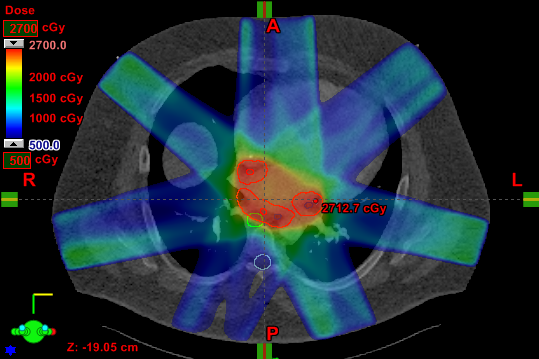
\includegraphics[scale=0.6]{Pat05_transverse.png}
 }
 \subfigure[Patient 2 : carbon ions (IMPT)]{
   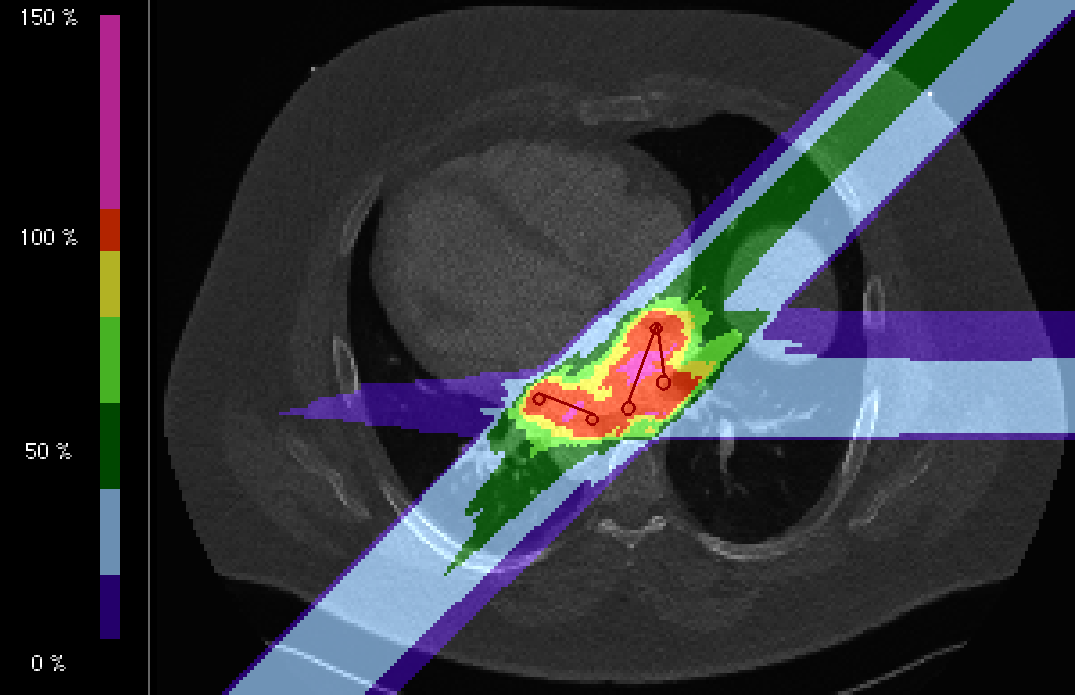
\includegraphics[scale=0.31]{Pat05_IMPT_5mmMargin_STATIC_slice38_cut_withLegend.png}}
%  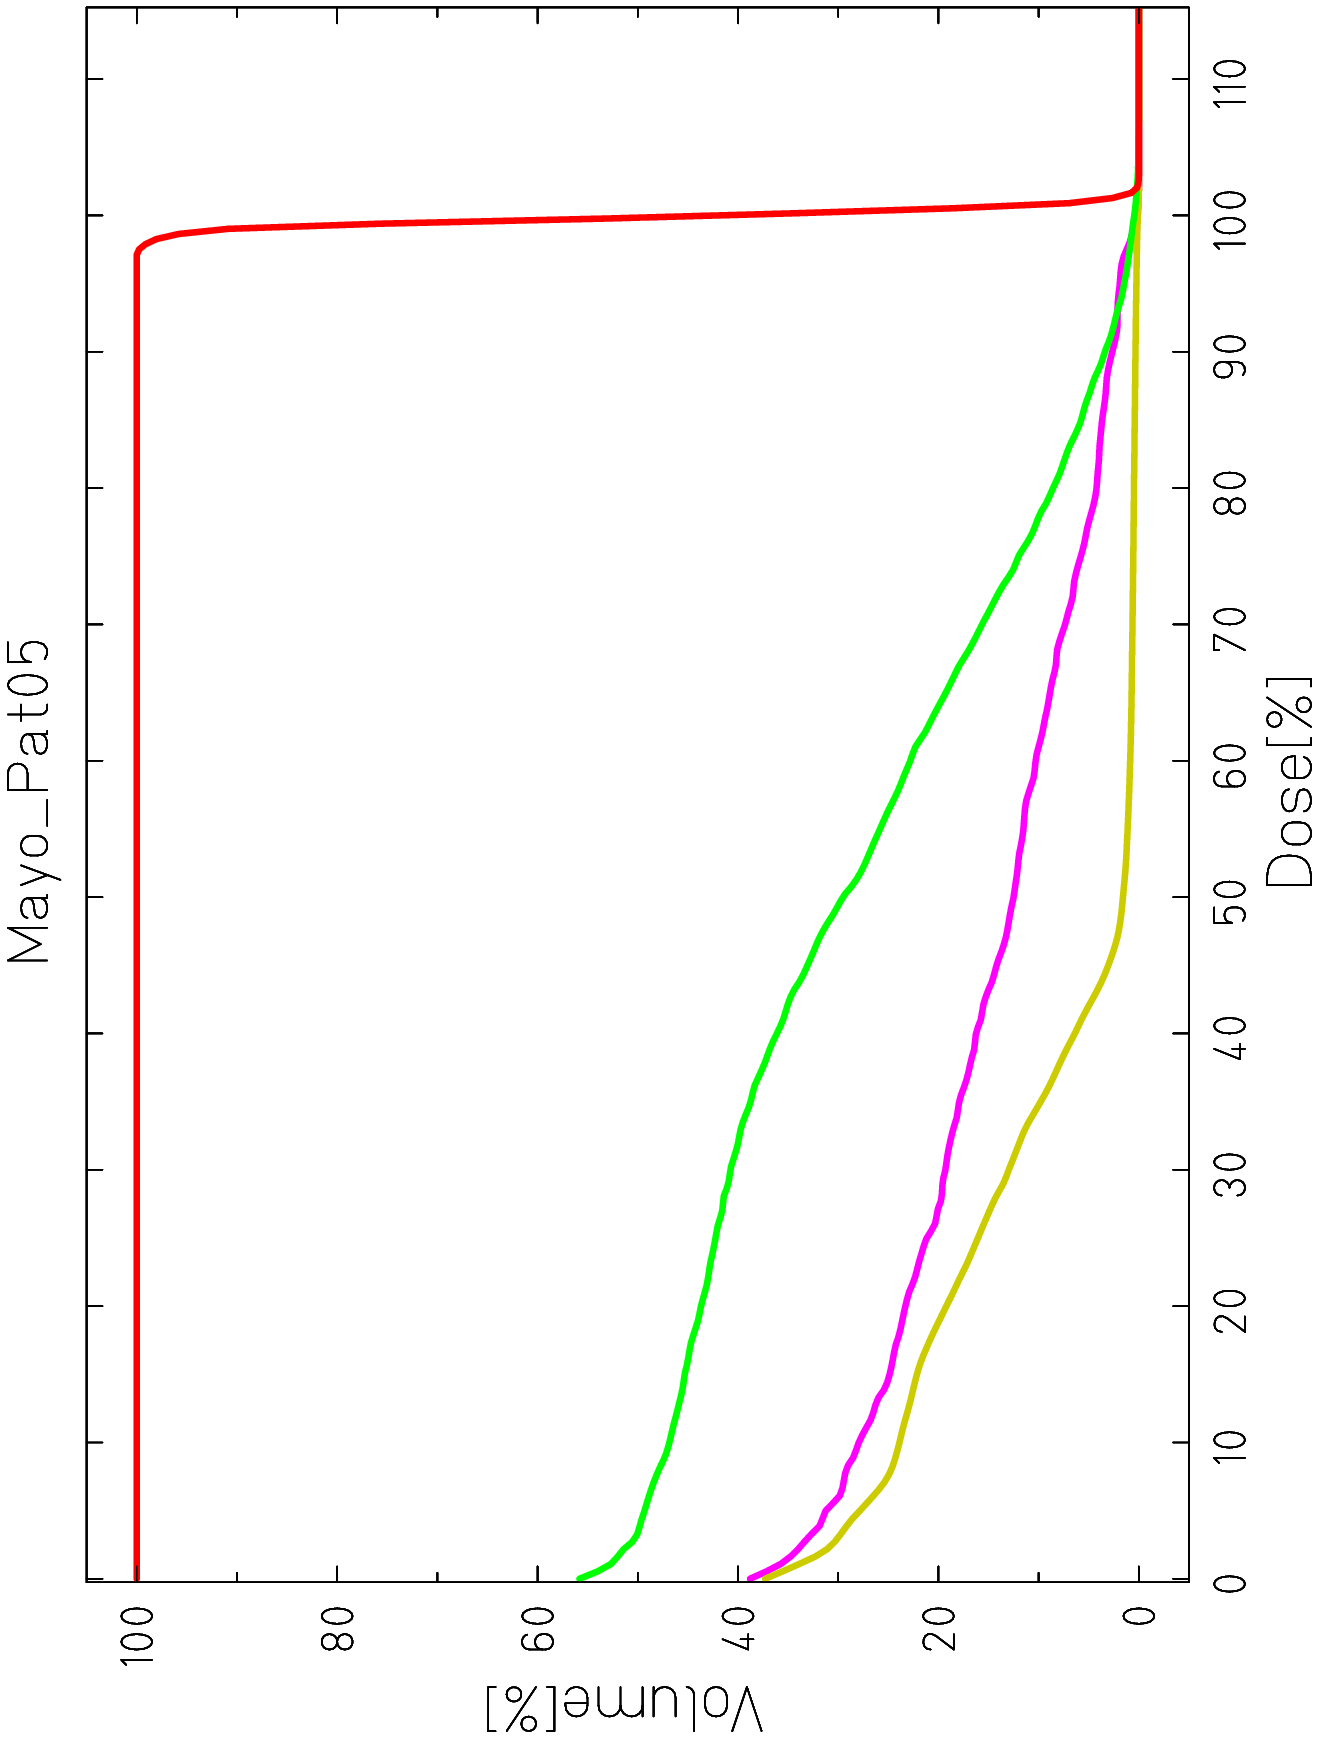
\includegraphics[scale=0.605]{Pat05_DVH.png}
%  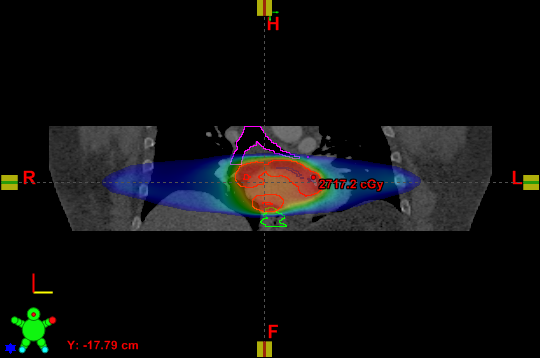
\includegraphics[scale=0.4]{Pat05_coronal.png}
%  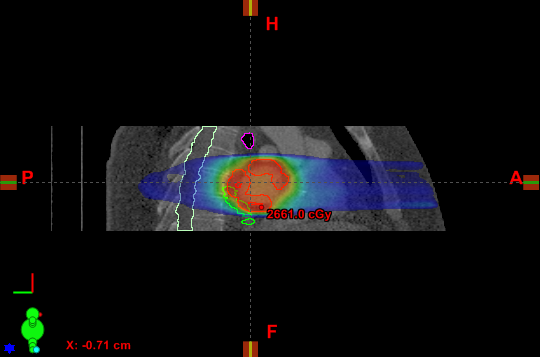
\includegraphics[scale=0.4]{Pat05_sagittal.png}
% }
\subfigure[Patient 4 : photons (IMRT)]{
 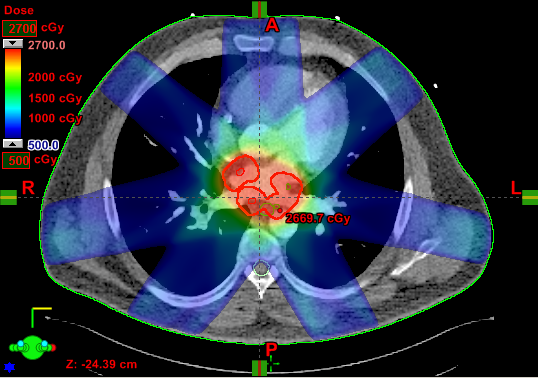
\includegraphics[scale=0.6]{Pat08_transverse.png}}
 \subfigure[Patient 4 : carbon ions (IMPT)]{
  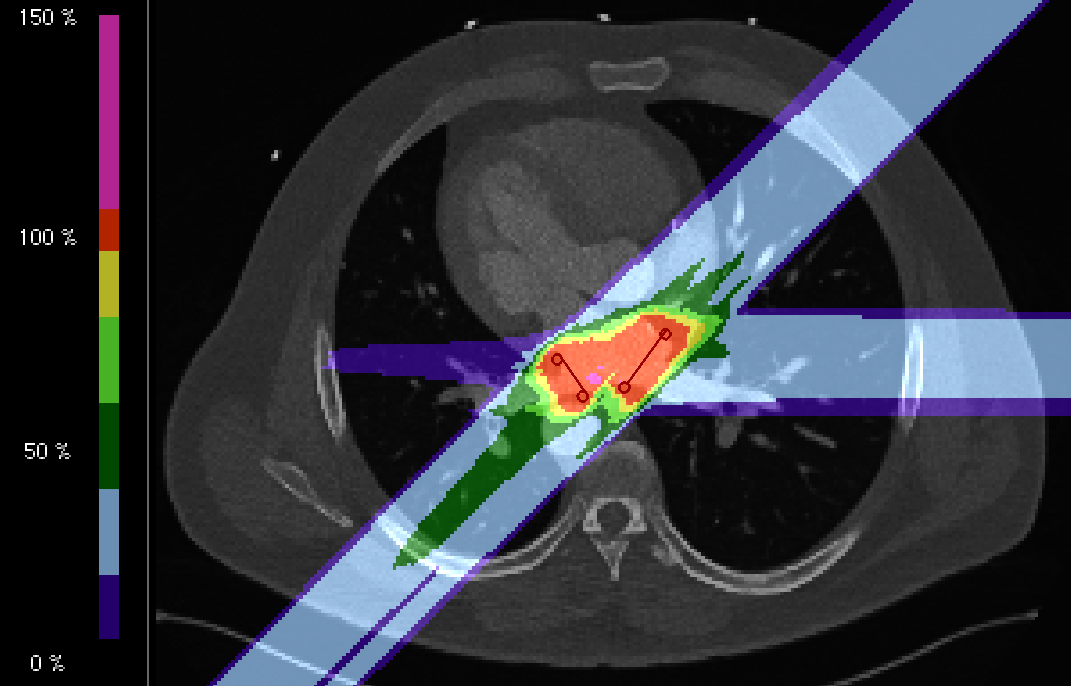
\includegraphics[scale=0.33]{Pat08_IMPT_5mmMargin_STATIC_slice43_cut_withLegend.png}}
%  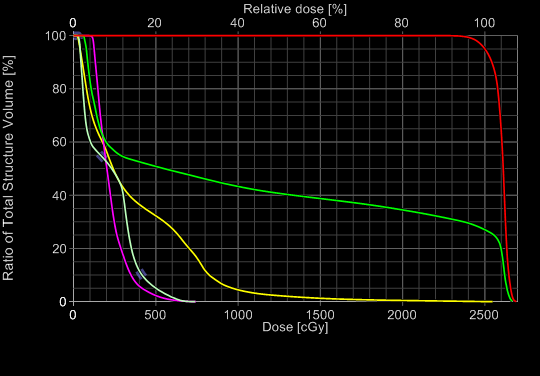
\includegraphics[scale=0.605]{Pat08_DVH.png}
% }
\caption{Comparison of dose cuts with photons (IMRT) and carbon ions (IMPT) treatment are shown for Patient 2 and Patient 4, respectively.} 
% Both treatments were carried out with an isotropic margin of 5mm on the CTV. 
% The corresponding DVHs are 
% shown on the right, where the PTV dose deposition is displayed in red, the dose to the esophagus in green, the trachea 
% dose in pink, the lung dose in yellow and the spinal cord dose in light green. 
% Photon treatment plans are courtesy of Dr.Amanda Deisher, Mayo Clinic, USA. The display of the CT data is mirrored in the photon 
% treatment planning screen shots (left) compared to the carbon ion treatment pictures (right).}
\label{dose_IMRT_vs_IMPT}
\end{figure}

% \newpage

\begin{table}[H]
\scriptsize
  \centering
  \caption{Dose-volume limits for OARs.}
  \begin{tabular}{|c|c||c|c|c||c|c|c|}
    \hline\hline
    Patient & OAR & Volume [cc] & Dose [Gy] & endpoint & IMRT [Gy] & IMPT (weak) [Gy] & IMPT (strong) [Gy]\\
    \hline
    2 & Aorta / great vessels & 10 & 31 & Aneurysm & 22.0 & 14.3 & 15.3 \\
    & Esophagus & 5 & 11.9 &  Stenosis / fistula & 24.6 & 22.5 & 7 \\
    & Heart & 15 & 16 & Pericarditis & 27.1 & 25 & 25.3 \\
    & Trachea & 4 & 10.5 & Stenosis / fistula & 0.8 & 4.3 & 3 \\
    \hline
    5 & Aorta / great vessels & 10 & 31 & Aneurysm & 21.3 & 8.5 & 6.3\\
    & Esophagus & 5 & 11.9 &  Stenosis / fistula & 20.2 & 18.5 & 3.5 \\
    & Heart & 15 & 16 & Pericarditis & 26.1 & 20.5 & 16.8 \\
    & Trachea & 4 & 10.5 & Stenosis / fistula & 0.2 & 0 & 0 \\  
    \hline\hline
  \end{tabular}
  \label{tab:dosevolume:photons:carbon}
\end{table}

\newpage

\vspace*{1.5cm}

\begin{figure}[H]
\begin{tikzpicture}
    \node (pic1) at (0,0) {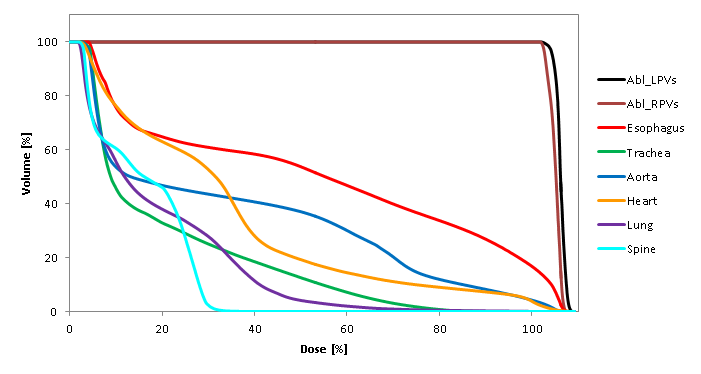
\includegraphics[scale=0.46]{Pat05_DVH_Amanda_withLegend.png}};
    \node (text1) at (0,-2.5) {(a) Patient 2 : photons (IMRT)};

    \node (pic2) at (8,0.08) {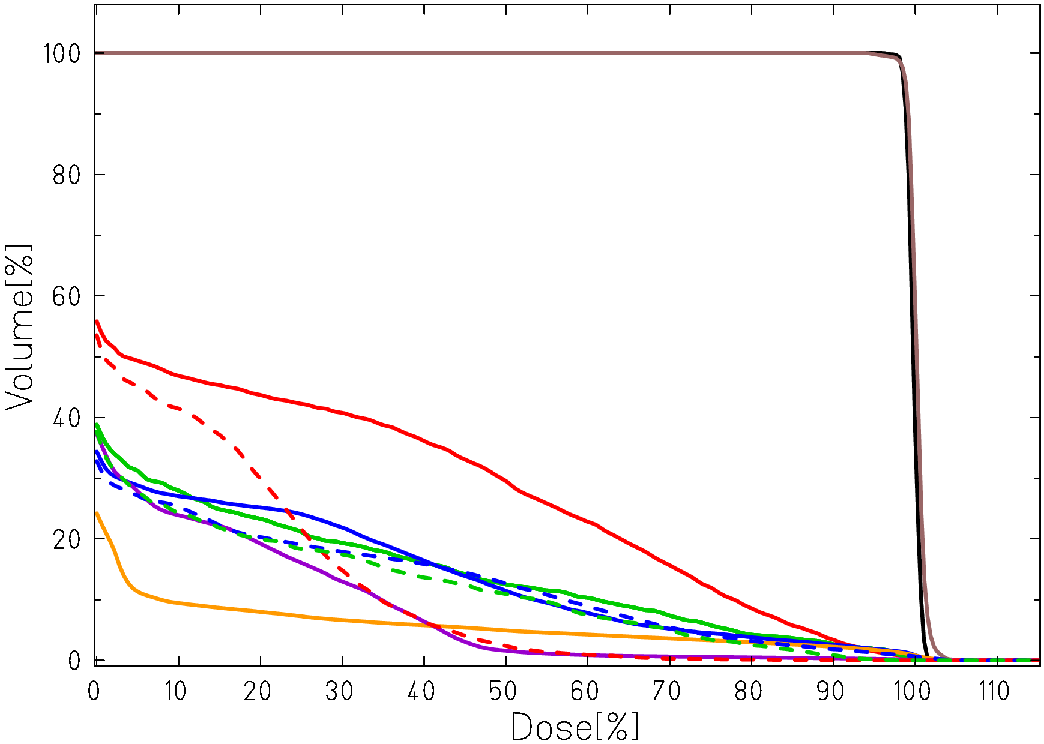
\includegraphics[scale=0.20]{Pat05_IMPT_VS_AMANDA_DVH_withOtherParameters_rotated.png}};
    \node (text2) at (8,-2.5) {(b) Patient 2 : carbon ions (IMPT)};
    
    \node (pic3) at (0,-5) {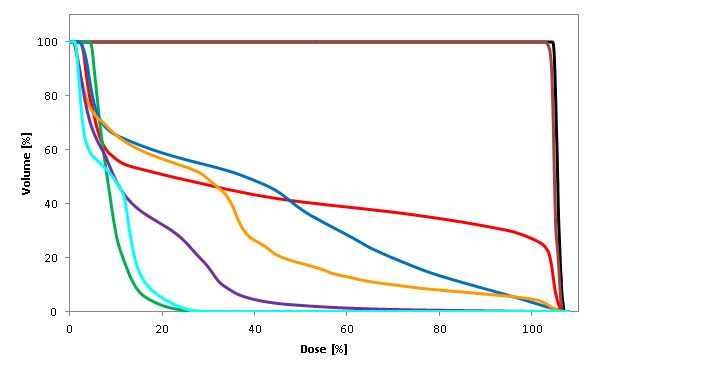
\includegraphics[scale=0.46]{Pat08_DVH_Amanda_forLegend.png}};
    \node (text3) at (0,-7.5) {(a) Patient 5 : photons (IMRT)};
    
    \node (pic4) at (8,-4.92) {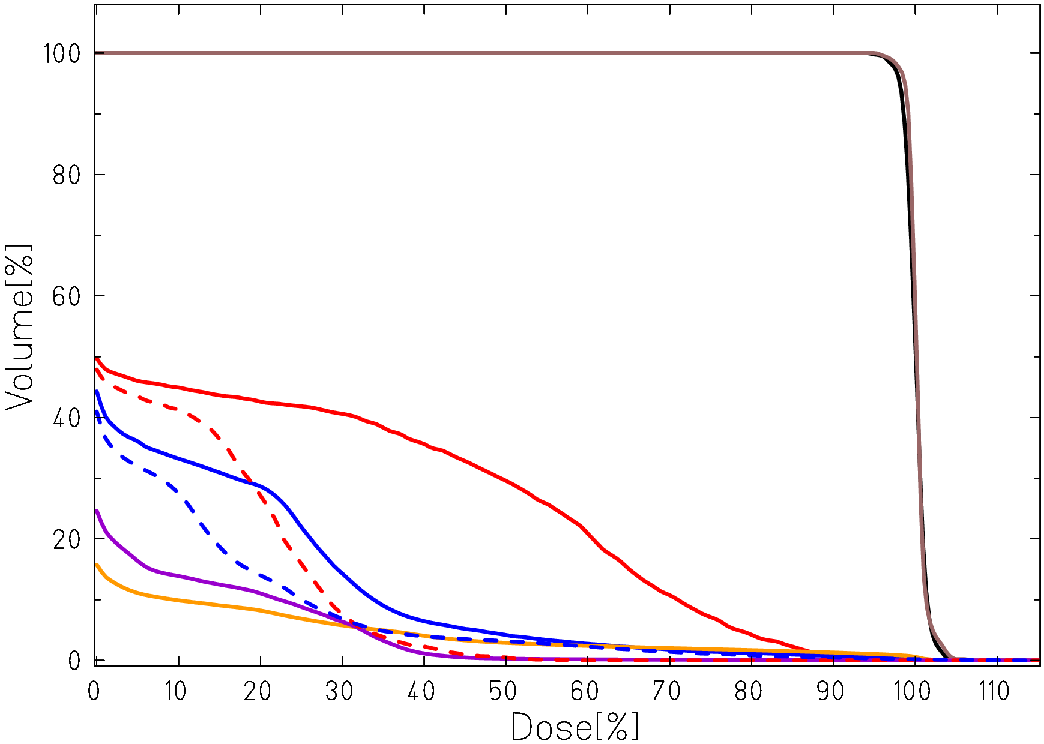
\includegraphics[scale=0.20]{Pat08_IMPT_VS_AMANDA_DVH_withOtherParameters_rotated.png}};
    \node (text4) at (8,-7.5) {(b) Patient 5 : carbon ions (IMPT)};
\end{tikzpicture}
\caption{Comparison of DVHs are displayed for a treatment with photons (IMRT) versus carbon ions (IMPT). 
Target dose deposition are shown in black for the LPVs and brown for the RPVs, the dose to the esophagus is displayed in red, the trachea dose 
in green, the aorta dose in blue, the heart dose in orange, the lung dose in purple and the spinal cord dose in light blue. Photon treatment 
plans are courtesy of Dr. Amanda Deisher, Mayo Clinic, USA. For the carbon ion treatment plans different IMPT parameters are shown, where 
a better sparing of the esophagus is achieved with stronger limitation parameters, shown in dashed lines.}
\label{dvh_patients_photon_vs_carbon}
\end{figure}

\begin{table}[H]
  \centering
  \caption{Specific integral dose (SID).}
  \begin{tabular}{|c|c||c|c|}
    \hline\hline
    Patient & Body Contour Volume [cc] & IMRT: SID [Gy*cm$^{3}$]& IMPT: SID [Gy*cm$^{3}$] \\
    \hline
    2 & 16,593 & 62,578 & 109 \\
    \hline
    5 & 10,735 & 35,711 & 78 \\
    \hline\hline
  \end{tabular}
  \label{tab:SID}
\end{table}

\newpage

\subsubsection{Porcine data}

Photon treatment plans for the irradiation of the AV node were carried out on different CT phases for all four porcine data sets (see chapter XXX) as a 
five field IMRT treatment (see figure \ref{dose_porcine_photon_vs_carbon}) with 6MV photons. The CT phases were reduced from twenty motion phases to ten. 
The planning phase was chosen depending on the resulting ITV volume in order to keep it as small as possible. This resulted in an treatment 
planning on 70\% of the cardiac phase for Pig 1, on 20\% for Pig 2, 0\% (reference phase) for Pig 3 and 70\% for Pig 4. The delivery was also 
planned as a single fraction irradiation of 25Gy. For the ITV volumes additional 3mm isotropic expensions were used, resulting in the final 
PTV. For a fair comparison the shown carbon ion results were calculated on the same CT scan phases. The plans are SFUD irradiations with an 
isoptropic safety margin of 5mm to the CTV. The SFUD carbon ion plans were generated with two opposing beam channel directions (see chapter 
XXX). The target volume as well as the contours of the OAR were kept identical in both deliveries, enabling a direct comparison of the 
treatment planning outcome.\newline
\newline
The sparing of the OARs are shown both in the resulting dose-volume deposition 
in table \ref{tab:pig:dosevolume:photons:carbon} as well as in the comparison of the resulting DVHs for photons and carbon 
ions (see figure \ref{dvh_porcine_photon_vs_carbon}). Due to the inverse depth-dose profile of carbon ions a reduced number of beam 
channel entry directions is feasible, resulting in a better sparing of the OARs compared to an irradiation of the AV node with photons. 
Due to the used beam channel directions it can be seen that the esophagus as well as the trachea are not receiving any dose deposition. 
The dose deposition in the aorta is negligible, resulting in an irradiated volume of less than 10cc. Also the heart itself is much better 
spared with carbon ions, resulting in no dose-volume-limit exceeding irradiation for this structure. For photons on the other hand 
the limit is exceeded in three out of the four studied data sets. It should be noted that the analyzed heart volume excludes the irradiated 
AV node volume and hence the highest dose deposition, the target dose of 25Gy physical dose.\newline
\newline
Also in the porcine data sets the body was only partially displayed on the CT scans and hence no density information could be derived for the 
calculation of the integral dose. The specific integral dose for both treatment delivery techniques were determined also for these cases. 
Thereby the sum over all dose volume products was calculated for the body contour volume. The results are shown in 
table \ref{tab:SID:pigs} and it can be seen that the absorbed energy to the body volume can be drastically reduced with carbon ions 
compared to photons.

\newpage

\begin{figure}[H]
\centering
\subfigure[Pig 3 : photons (IMRT)]{
 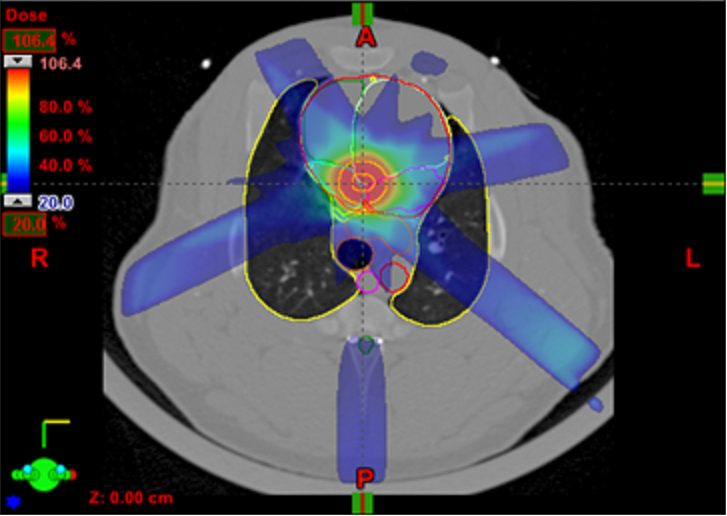
\includegraphics[scale=0.46]{L976_IMRT_Limin.png}
 }
 \subfigure[Pig 3 : carbon ions (SFUD)]{
%   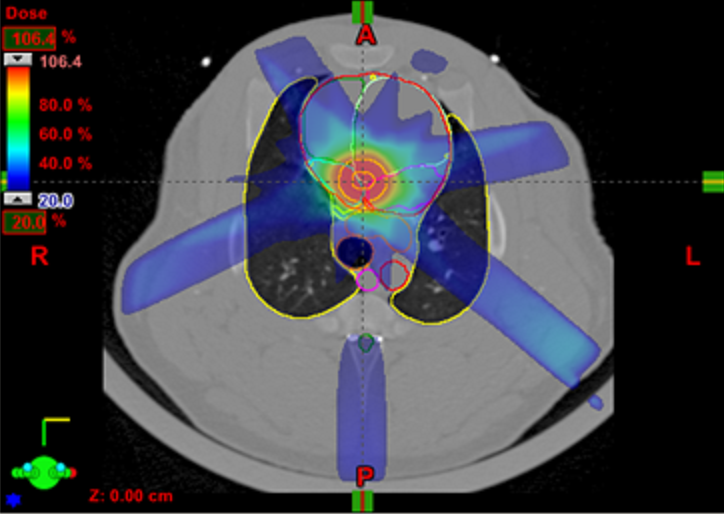
\includegraphics[scale=0.4]{L976_3Ddosis_Limin.png}
   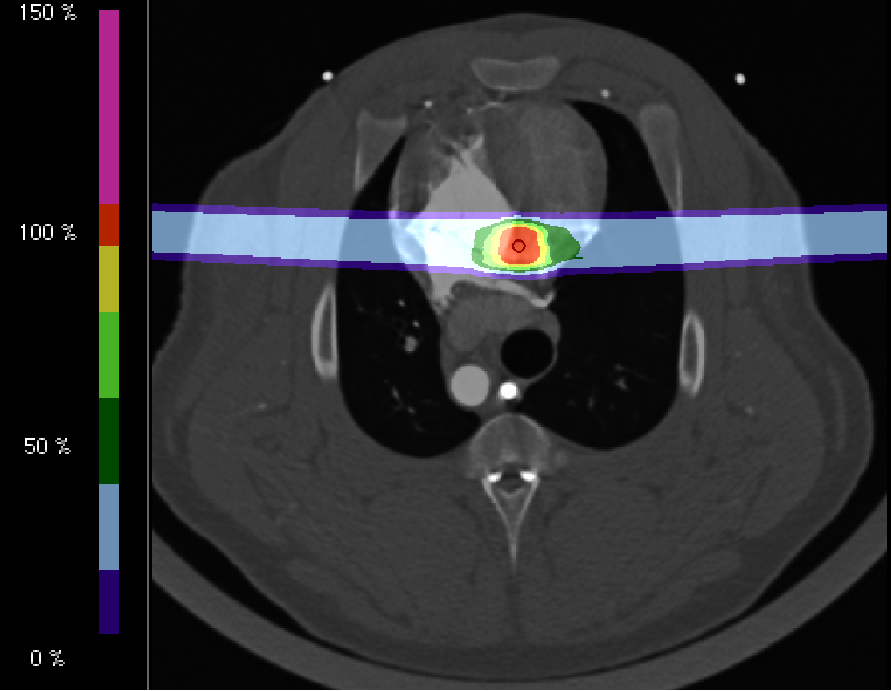
\includegraphics[scale=0.34]{L976_static_CTV_slice37_cut.png}
   }
\caption{Comparison of dose cuts with photons and carbon ions treatment are shown for Pig 3. The photon delivery was planned as IMRT treatment 
and the carbon irradiation as SFUD irradiation, respectively. 
Photon treatment plans are courtesy of Dr.Limin Song, Mayo Clinic, USA.}
\label{dose_porcine_photon_vs_carbon}
\end{figure}

\begin{table}[H]
\scriptsize
  \centering
  \caption{Dose-volume limits for OARs.}
  \begin{tabular}{|c|c||c|c|c||c|c|c|}
    \hline\hline
    Pig & OAR & Volume [cc] & Dose [Gy] & endpoint & IMRT (photons) [Gy] & SFUD (Carbon) [Gy] \\
    \hline
    1 & Aorta / great vessels & 10 & 31 & Aneurysm & 1.1 & 0.0 \\
    & Esophagus & 5 & 11.9 &  Stenosis / fistula & 0.2 & 0.0 \\
    & Heart & 15 & 16 & Pericarditis & 18 & 6.3 \\
    & Trachea & 4 & 10.5 & Stenosis / fistula & 6.5 & 0.0 \\
    \hline
    2 & Aorta / great vessels & 10 & 31 & Aneurysm & 2.1 & 0.0 \\
    & Esophagus & 5 & 11.9 &  Stenosis / fistula & 0.4 & 0.0 \\
    & Heart & 15 & 16 & Pericarditis & 16.1 & 6.5 \\
    & Trachea & 4 & 10.5 & Stenosis / fistula & 2.6 & 0.0 \\
    \hline
    3 & Aorta / great vessels & 10 & 31 & Aneurysm & 0.9 & 0.0 \\
    & Esophagus & 5 & 11.9 &  Stenosis / fistula & 0.3 & 0.0 \\
    & Heart & 15 & 16 & Pericarditis & 23 &  4.8 \\
    & Trachea & 4 & 10.5 & Stenosis / fistula & 0.2 & 0.0 \\
    \hline
    4 & Aorta / great vessels & 10 & 31 & Aneurysm & 0.7 & 0.0 \\
    & Esophagus & 5 & 11.9 &  Stenosis / fistula & 0.3 & 0.0 \\
    & Heart & 15 & 16 & Pericarditis &  14.3 & 7.3 \\
    & Trachea & 4 & 10.5 & Stenosis / fistula & 4.6 & 0.0 \\
    \hline\hline
  \end{tabular}
  \label{tab:pig:dosevolume:photons:carbon}
\end{table}

\begin{table}[H]
\footnotesize
  \centering
  \caption{Specific integral dose (SID).}
  \begin{tabular}{|c|c||c|c|}
    \hline\hline
    Pig & Body Contour Volume [cc] & IMRT (photons): SID [Gy*cm$^{3}$]& SFUD (Carbon): SID [Gy*cm$^{3}$] \\
    \hline
    1 & 6,121 & 5,237 & 11 \\
    \hline
    2 & 5,228 & 4,473 & 13 \\
    \hline
    3 & 5,209 & 6,157 & 15 \\
    \hline
    4 & 6,928 & 4,031 & 10 \\
    \hline\hline
  \end{tabular}
  \label{tab:SID:pigs}
\end{table}


\vspace*{-0.4cm}
\begin{figure}
\begin{tikzpicture}
    \node (pic1) at (0,0) {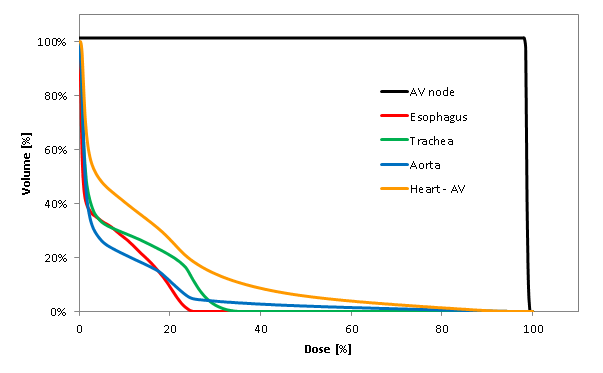
\includegraphics[scale=0.46]{L829_IMRT_DVH_Limin.png}};
    \node (text1) at (0,-2.5) {(a) Pig 1 : photons (IMRT)};
%     \node (text1) [below of pic1] {(a) Pig 1 : photons (IMRT)};

    \node (pic2) at (8,0.08) {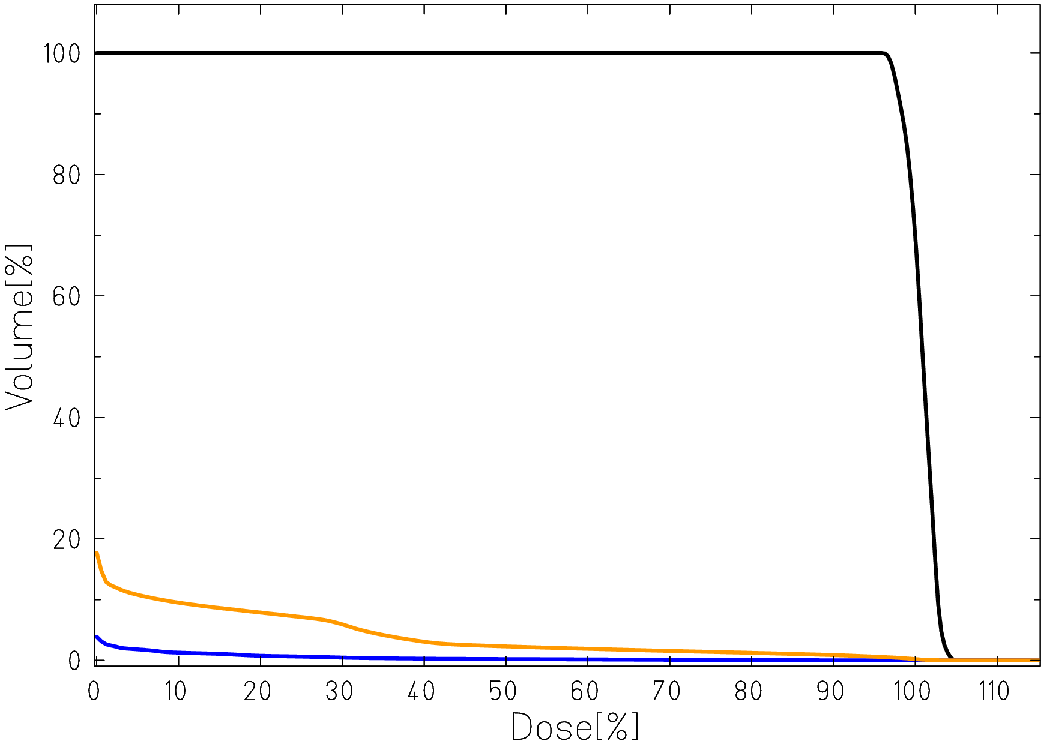
\includegraphics[scale=0.205]{L829_STATIC_VS_LIMIN_DVH_rotate.png}};
    \node (text2) at (8,-2.5) {(b) Pig 1 : carbon ions (SFUD)};
    
    \node (pic3) at (0,-5) {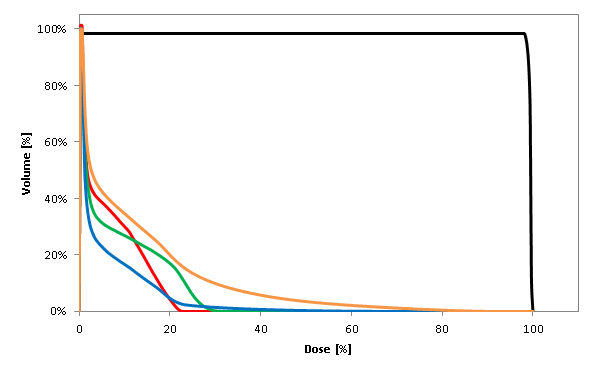
\includegraphics[scale=0.46]{L833_IMRT_DVH_Limin.png}};
    \node (text3) at (0,-7.5) {(a) Pig 2 : photons (IMRT)};
    
    \node (pic4) at (8,-4.92) {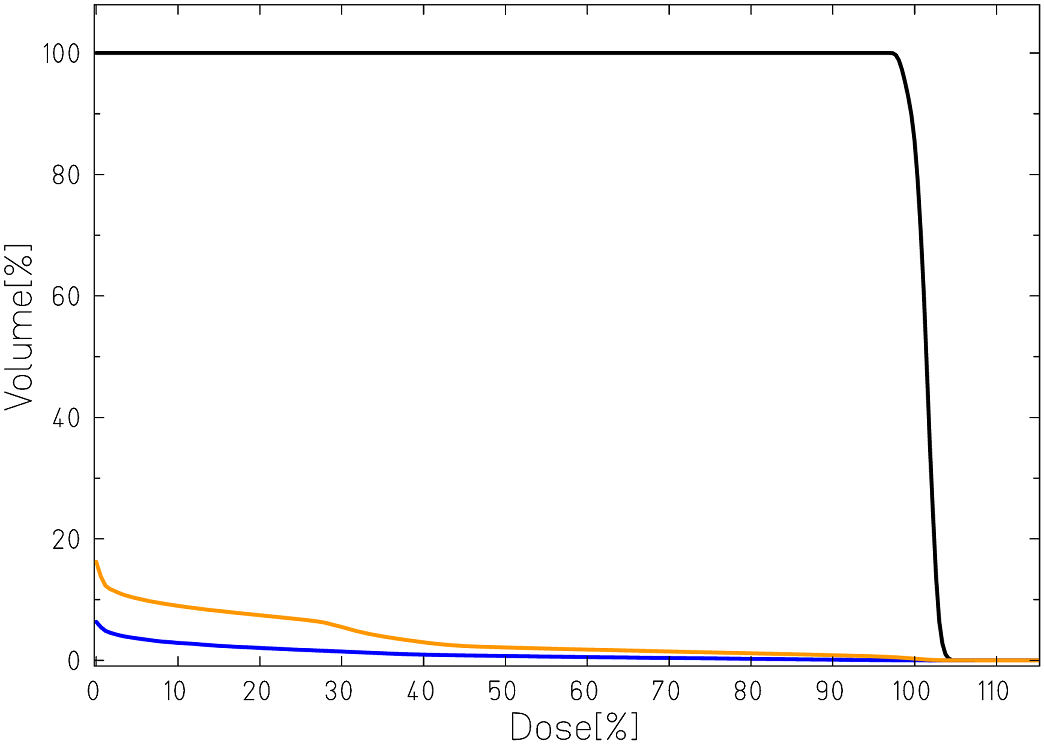
\includegraphics[scale=0.205]{L833_STATIC_VS_LIMIN_DVH_rotate.png}};
    \node (text4) at (8,-7.5) {(b) Pig 2 : carbon ions (SFUD)};
    
    \node (pic5) at (0,-10) {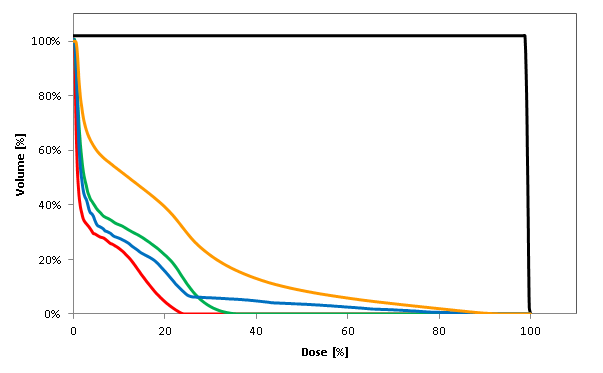
\includegraphics[scale=0.46]{L976_IMRT_DVH_Limin.png}};
    \node (text5) at (0,-12.5) {(a) Pig 3 : photons (IMRT)};
    
    \node (pic6) at (8,-9.92) {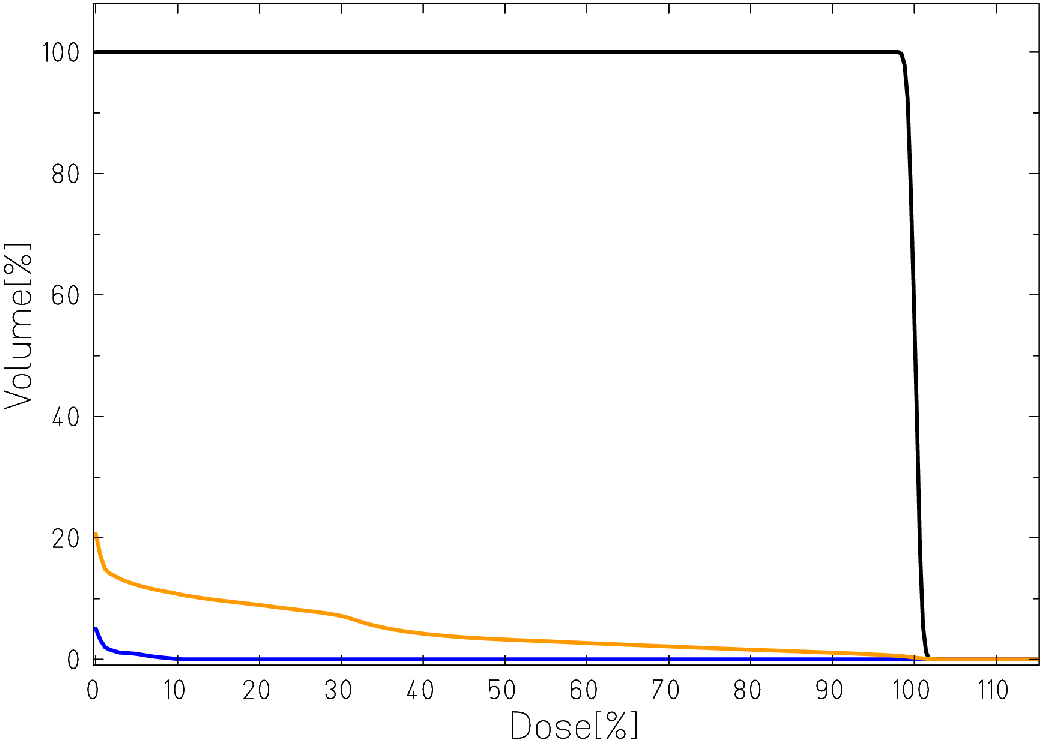
\includegraphics[scale=0.205]{L976_STATIC_VS_LIMIN_DVH_rotate.png}};
    \node (text6) at (8,-12.5) {(b) Pig 3 : carbon ions (SFUD)};
    
    \node (pic7) at (0,-15) {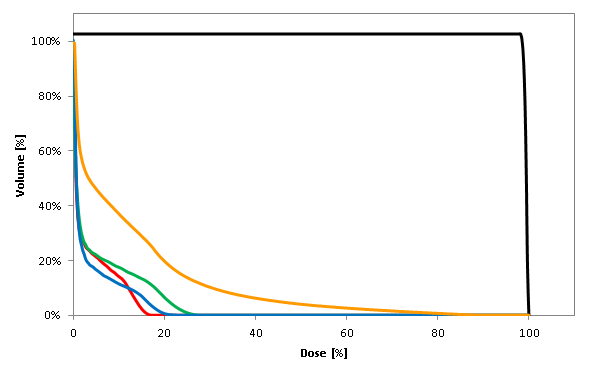
\includegraphics[scale=0.46]{L979_IMRT_DVH_Limin.png}};
    \node (text7) at (0,-17.5) {(a) Pig 4 : photons (IMRT)};   
    
    \node (pic8) at (8,-14.92) {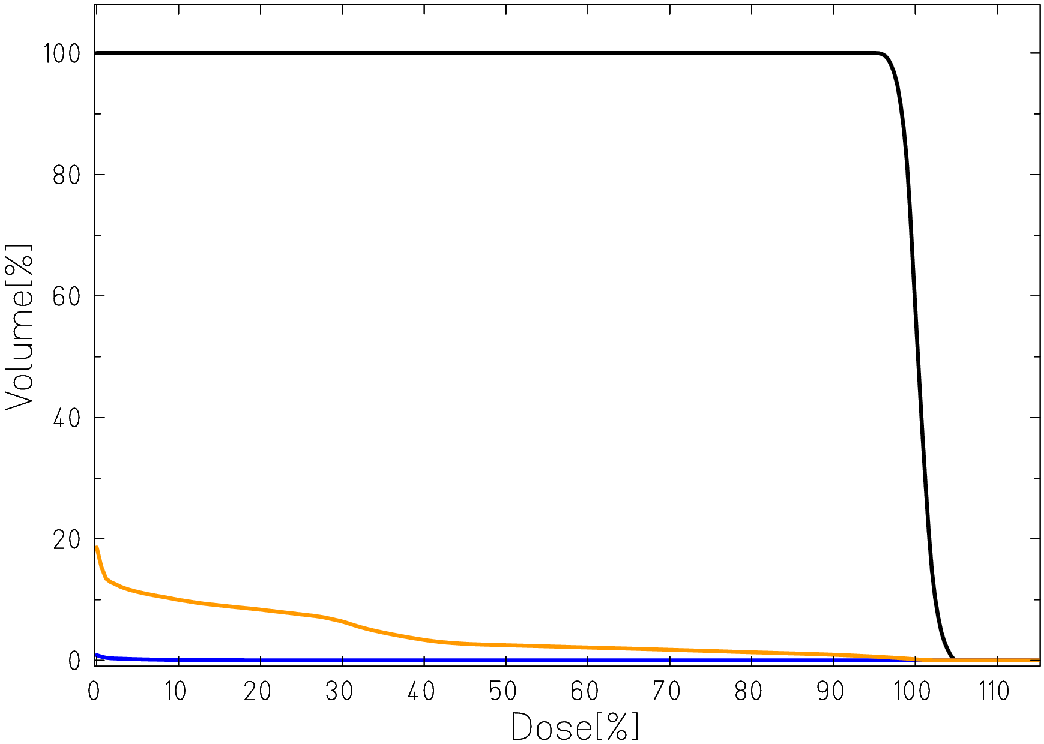
\includegraphics[scale=0.205]{L979_STATIC_VS_LIMIN_DVH_rotate.png}};
    \node (text8) at (8,-17.5) {(b) Pig 4 : carbon ions (SFUD)};

\end{tikzpicture}
    \caption{Comparison of DVH results with photons (left) and carbon ions (right). The photon delivery was planned as IMRT treatment 
and the carbon irradiation as SFUD irradiation, respectively. The target dose to the AV node is displayed in black, the dose to the 
esophagus in red, to the trachea in green, the aorta in blue and the irradiated heart (substracted the target area of the AV node) is shown 
in orange. Photon treatment plans are courtesy of Dr. Limin Song, Mayo Clinic, USA.}
\label{dvh_porcine_photon_vs_carbon}
\end{figure}

\newpage

% 
% \begin{figure}[H]
% \centering
% \subfigure[Pig 1 : photons (IMRT)]{
%  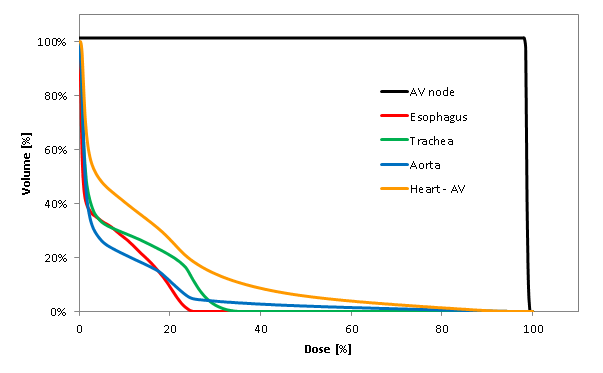
\includegraphics[scale=0.46]{L829_IMRT_DVH_Limin.png}
%  }
%  \subfigure[Pig 1 : carbon ions (SFUD)]{
%    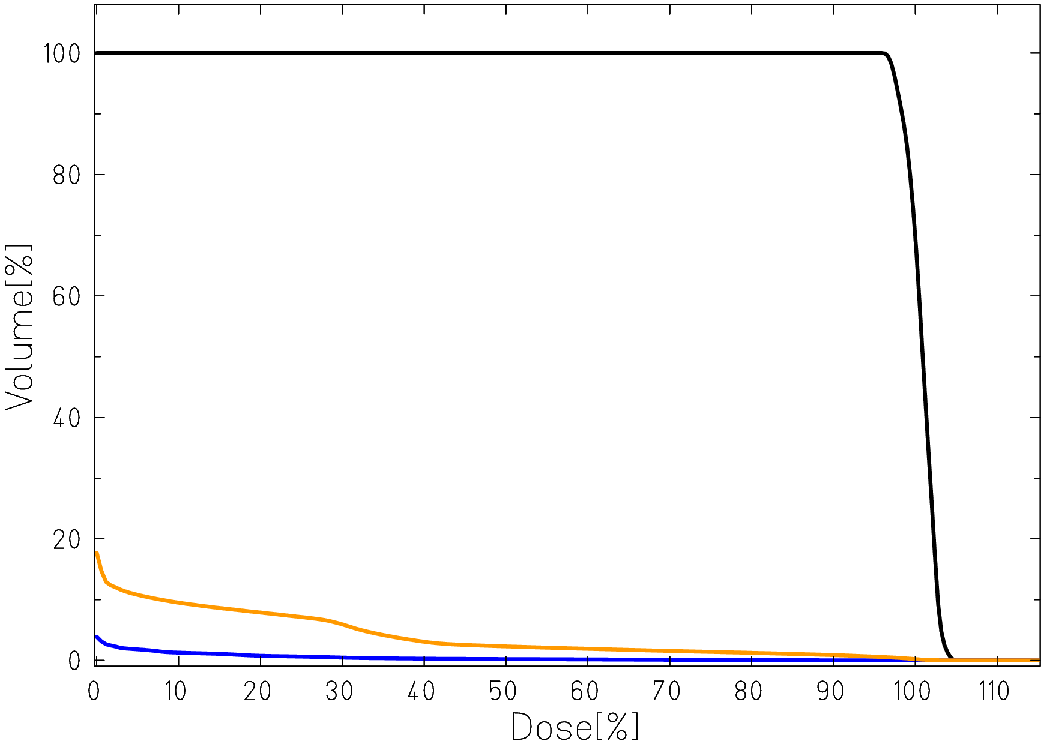
\includegraphics[scale=0.2]{L829_STATIC_VS_LIMIN_DVH_rotate.png}
%    }
%    \subfigure[Pig 2 : photons (IMRT)]{
%  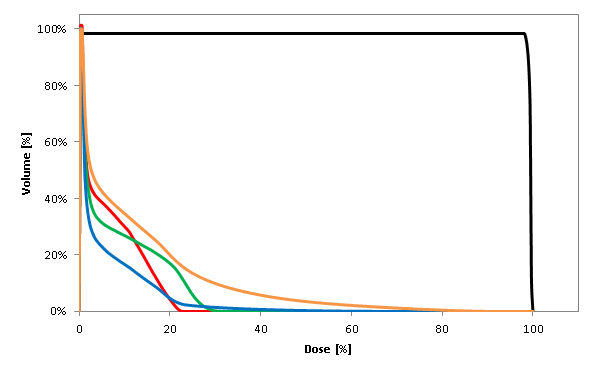
\includegraphics[scale=0.46]{L833_IMRT_DVH_Limin.png}
%  }
%  \subfigure[Pig 2 : carbon ions (SFUD)]{
%    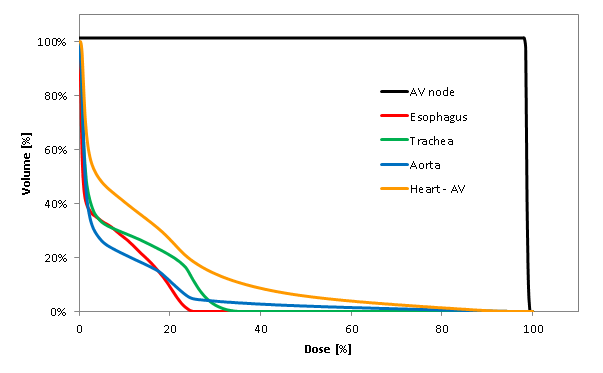
\includegraphics[scale=0.46]{L829_IMRT_DVH_Limin.png}
%    }
%    \subfigure[Pig 3 : photons (IMRT)]{
%  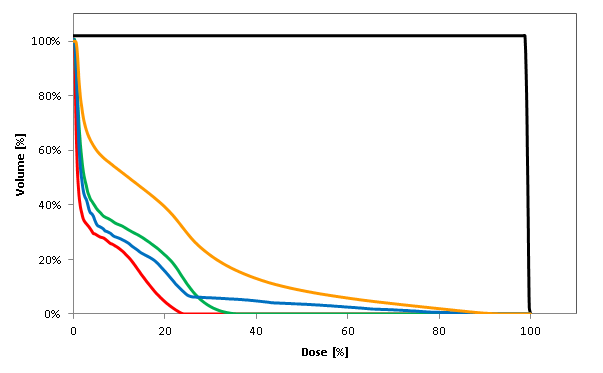
\includegraphics[scale=0.46]{L976_IMRT_DVH_Limin.png}
%  }
%  \subfigure[Pig 3 : carbon ions (SFUD)]{
%    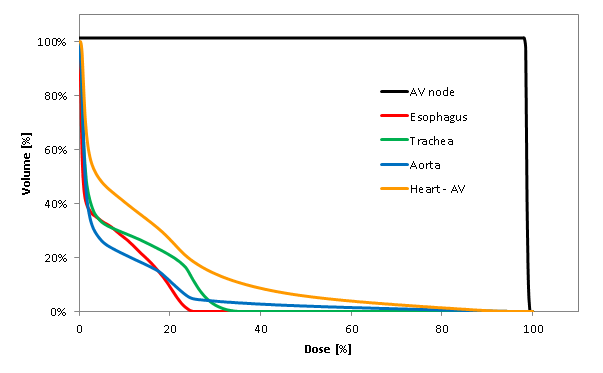
\includegraphics[scale=0.46]{L829_IMRT_DVH_Limin.png}
%    }
%    \subfigure[Pig 4 : photons (IMRT)]{
%  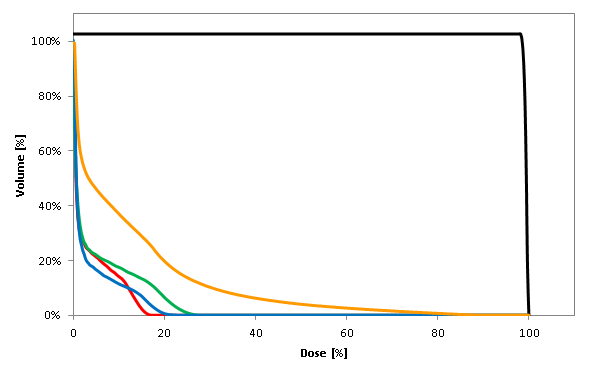
\includegraphics[scale=0.46]{L979_IMRT_DVH_Limin.png}
%  }
%  \subfigure[Pig 4 : carbon ions (SFUD)]{
%    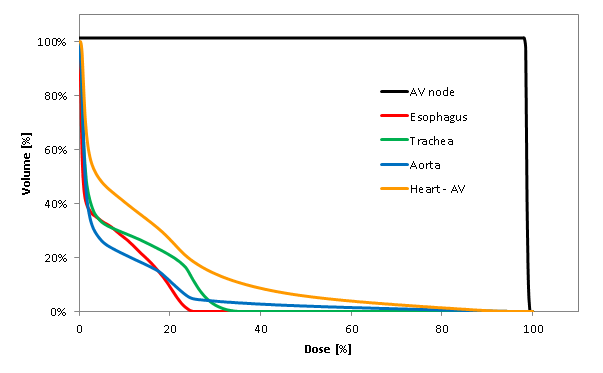
\includegraphics[scale=0.46]{L829_IMRT_DVH_Limin.png}
%    }
% \caption{Comparison of DVH results with photons and carbon ions treatment. The photon delivery was planned as IMRT treatment 
% and the carbon irradiation as SFUD irradiation, respectively. The target dose to the AV node is displayed in black, the dose to the 
% esophagus in red, to the trachea in green, the aorta in blue and the irradiated heart (substracted the target area of the AV node) is shown 
% in orange. Photon treatment plans are courtesy of Dr.Limin Song, Mayo Clinic, USA.}
% % \label{dvh_porcine_photon_vs_carbon}
% \end{figure}



\section{Motion of cardiac volumes}
\label{diss:motion}

Target volumes in the heart move on one hand due to the respiration of the patient, a motion with a large amplitude and large period, and on 
the other hand due to heartbeat, a motion with a small amplitude and small period. Even though both motion occur simultaneously in  
patients, they were studied independently in the here presented treatment planning studies. 

% - atmung versucht welche bewegung in pv
% - herzschlag verursacht welche bewegung in pv 
% 
% - im verlgeich: herzschlag verursacht welche bewegung in pv
% - schweine rest target volumen bewegung
% 
% - mmt needed

\subsection{PVs motion in humans}

The motion of PVs ablation sites in humans due to respiration were studied based on respiratory gated time resolved computed tomographies 
(4DCTs) of nine lung cancer patients, recorded for radiotherapy at MD Anderson Cancer Center (MDACC), USA. The heartbeat influence was studied 
on cardiac gated 4DCTs of five AF patients, recorded at Mayo Clinic, USA. 

\subsubsection{Due to respiration}

The movement of the ablation sites of the PVs were studied in the three motion directions (superior-inferior (SI), anterior-posterior (AP) 
and left-right (LR)) as well as for the absolute displacment. Different studies concerning the PVs displacment due to respiration can also 
be found in literature \cite{Ect08} \cite{Nos05}, as breathing displacement is also relevant for cather ablation due to the reduction in catheter 
tip contact force \cite{Kum12}. In the here studied patient cohort the SI direction was found to be the biggest motion 
direction with a mean displacment of up to 1cm, while AP and LR are almost negligible with a mean motion of less than 2mm. 
Moreover, the motion of the LPV and RPV are comparable in SI direction. In the other directions the difference between the two cardiac sites is 
more pronounced, so that e.g. the LPV move more in anterior direction. In 
LR direction a significant difference between LPV and RPV motion was found, where the mean displacement of the LPV is almost double compared 
to the RPV. 

\subsubsection{Due to heartbeat}

The motion of the ablation sites for the PVs was studied for the left and right structures, respectively, in the three above stated motion 
directions. Only a small mean absolute displacement over all patients of less then 3mm was observed. The biggest absolute displacment 
reached a mean value of up to (6.5 $\pm$ 3.0)mm in one patient case for the RPV and (5.5 $\pm$ 3.1)mm for the LPV. 
No dominant motion direction was found, even though a tendency to a bigger motion in AP direction could be assumed. Furthermore, no motion 
pattern could be derived from the five studied patient data sets, 
indicating that the underlying motion causing the PV ablation sites to move is much more complex and the result of different motion influences. 
For further studies concerning the PV displacement due to heartbeat, the reader should be refered to Lickfett et al. \cite{Lic05} and Patel et al. \cite{Pat08}. 

\subsection{Motion in porcine due to heartbeat}

The motion of different potential cardiac ablation sites (AV node, CTI and PVs) were studied in pigs based on cardiac gated 4DCTs of four 
swines, recorded at Mayo Clinic, USA. The acquired CT scans were both native and contrast enhanced. It was found that native CT scans 
do not enable an assessment of the cardiac target volume displacement due the low contrast between the cardiac muscle and the contained blood. 
Analysis was hence carried out on the contrast enhanced CT scans. Concerning the motion of the three studied potential target sites 
it could be stated that the PVs moved to the smallest extent (maximal displacement of up to 5mm), followed by the AV node (maximal 
displacement of up to 6mm) and that the CTI moved the most (maximal displacement of 7mm). It was speculated that 
this is due to the location of the volumes, where a proximer location on or near the ventricles lead to a larger movement. 
Even though also in the porcine data sets no maximal motion phase or motion pattern could be observed due to heartbeat it was found that the displacement was 
shallower between certain motion phases (motion phase 6 to 13) and hence, contrary to the studied human data, gating could be an optional 
motion mitigation technique. Moreover, in comparison to the human data, the displacement in AP direction in the porcine data was clearly 
larger than in the other two studied directions. 

% - vergleich bewegung pv : human porcine


\section{Contrast enhanced CT scans}
\label{ceCT}

Particle treatment planning needs to be carried out on native CT scans in order to obtain the correct range information \cite{Jaek01}. In case 
of the intended irradiation of cardiac target volumes it was found that native CT scans do not provide sufficient contrast between the  
heart muscle and the contained blood. As stated, the motion information can thus only be accessed from contrast-enhanced CT scans. 
It needs to be studied if the displacement vector field obtained from registration on the contrast enhanced CT scans yield a good enough 
agreement when directly used on the native data sets for the actual treatment planning. 
The resulting range uncertainties need to be carefully considered, especially regarding the dose to critical structures like the esophagus. 
Analog to studies by e.g. el Bentefour et al. \cite{Ben12}, where in vivo range verifications were 
successfully achieved with a small dose deposition (<0.5cGy) in silicone diodes, a possible solution could be to predeposit the resulting 
treatment plan with a small dose in the order of mGy. By placing such an detector with a catheter inside the patient, either in front of 
or inside the esophagus, it would allow to test for range of the planned energies and hence for potential miscalculation or 
interfractional changes of the organs. Range uncertainties to the target area could furthermore be corrected before irradiation with the 
total single fraction dose. By using in-beam PET monitoring with $^{11}$C and $^{10}$C fragments (see Introduction, chapter 
XXX) it would be possible to irradiate only a small dose of cGy and detect the range and position uncertainties. This was already carried 
out in XXX!!!! (hier pilotschuss paper wenn ich es denn mal finde). 
The accuracy of PET monitoring for ion range determination was studied by Fiedler et al. \cite{Fie10} for more than 80 of the 400 patients 
irradiated in the GSI pilot project. It was stated that in-beam PET method demonstrated a high sensitivity for the 
detection of range deviations and would thus be beneficial for the here presented treatment modality. 


\section{Motion mitigation techniques}
\label{diss:mmt}

Due to the large motion of the PV ablation sites induced by the respiratory motion in the studied patient cohort, interplay was oberved to 
lead to strong underdosage, so that in some cases only V95=70\% was achieved with no safety margin and V95=80\% with safety margins of 
5mm. Due to the large motion amplitude of more than 1cm gating was studied as potential motion mitigation technique (see section \ref{diss:resp:mmt}). 
For the displacements induced by heartbeat a smaller motion of less than 1cm was observed in all studied human data, so that rescanning was studied 
as an adequate motion mitigation technique for this case. As expected, the interplay effect in this case was smaller than for respiration, 
with minimal underdosages of V95=85\% for no safety margin and a minimal V95 of 92\% for 5mm and 7mm margin, respectively. 
Even though this underdosage with safety margin already yields a clinically acceptable dose coverage the usage of an additional motion 
mitigation technique leads to a more robust treatment 
delivery, as is stated in \ref{diss:hb:mmt}. For the porcine data, where the motion influence of the heartbeat on the AV node target volume 
was studied and only a single margin of 5mm was used, the interplay effect led to larger minimal underdosages of 56\% in some of the studied 
pig data sets. Hence the usage of rescanning as motion mitigation technique was also needed in this case. 

% - wie gross interplay?
% - gating fuer atmung
% - rescanning fuer herzschlag
% 
% - vergleich rescanning human porcine? auch wenn unters target und dadurch unfair

% - !!! vergleich mit bestrahlung cyberheart und luebeck

\subsection{Respiratory motion}
\label{diss:resp:mmt}

% -apnea

In the animal model studies by Sharma et al. \cite{Sha10} the target displacement due to respiration was tracked with the CyberKnife 
system. In the study by Blanck et al. \cite{Bla13} an ITV approach was used for the respiratory motion. Here, gating was used as a potential 
motion mitigation technique. It is suited for larger target displacments, since only a fraction of the motion cycle is used. Typically only 
the displacements around end exhale are used, enabling a more robust delivery with only a small amount of residual motion. 
To this date, gating is already used in ion beam centers with passive particle delivery \cite{Min00} as well as in IMRT treatments 
in photon centers \cite{Kea06}. A pilot study with scanned carbon ions was recently conducted on liver patients at HIT by using gating and 
abdominal compression \cite{Ric12}. In the here studied case, gating resulted to be an adequate motion mitigation technique so that underdosages could be increased up to 
a minimum of 98\% for all studied safety margins and patient cases. Even in cases with no safety margin underdosage could be increased to a 
minimum of 94\%. It can nevertheless be stated that safety margins, which are needed in order to account for e.g. position inaccuracies, 
improved the outcome and made the delivery more robust. It was furthermore studied in two patient data sets if the treatment outcome improved 
when rescanning was applied for the residual motion inside the gating window. This is proposed as phase-controlled rescanning by Furukawa et 
al. \cite{Fur07}. It resulted in a marginal improvement compared to only gating, whereas no improvement was observed when using more than ten 
rescans. Since the irradiation of the PV ablation sites were also studied to include rescanning as mitigation for heartbeat motion, the 
combination of these two techniques will be naturally achieved. Concerning the treatment time it was expected that gating would increase the 
treatment time dependent on the used gating window. Since an irradiation on about 30\% of the motion cycle was used, the treatment 
resulted into a delivery time of about 30min with a high intensity of 55.000 minimum particle and for a safety margin of 3mm. This was 
found for the HIT beam parameters, where a relatively short time for an energy change is needed. Nevertheless the particle intensity can 
be further increased, leading to an even further reduced treatment time. Compared to the radiofrequency ablation procedure which takes up to 
a couple of hours, and to the photon irradiation of up to two hours \cite{Sha10} , the treatment time is drastically reduced. 
An alternative to gating could be the usage of apneic oxygenation, which is currently used at the Rinecker Proton Therapy Center in Munich 
\cite{Ber11} for the treatment of tumors in the upper abdomen and thorax. This approach will also be used in the planned animal experiments 
with pigs which will be carried out at GSI in the summer of 2014. 

\subsection{Heartbeat motion}
\label{diss:hb:mmt}

% - rescanning wird besser je groesser margin und je mehr rescans
% - andere rescanning methoden: breath sampled, (phase based)

In the animal model studies by Sharma et al. \cite{Sha10} and by Blanck et al. \cite{Bla13} an ITV approach was used for the heartbeat motion. 
In the here presented study rescanning was used as a motion mitigation technique for heartbeat motion, both in human as well as for 
the porcine data sets. Especially in human data only rescanning seemed to be an adequate technique due to the lack of a motion pattern 
or a region of shallower motion. For the porcine data on the contrary, cardiac gating might be another option, which needs to be investigated. 
In the human data it was found that the dose coverage was higher than 99\% in about 96\% of the studied cases with safety margins over 3mm. 
This result could be even further improved if ten or more rescans were applied. Nevertheless it can be argued that five rescans already 
yield a very good dose deposition in the target volume. For the porcine data and the studied AV node ablation it was found 
that the dose coverage was higher than 99\% in 94\% of the studied cases with a safety margin of 5mm. Even though this finding could be 
slightly improved with ten rescans or higher, the finding indicates that five rescans are already sufficient to enable a robust and 
stable irradiation of the cardiac target volume in the presence of heartbeat. Due to the high single dose the resulting intensity per rescan 
is expected to be large and hence the application should be feasible without further prolonging the treatment time. 
All the studied rescanning results were obtained for slice-by-slice rescanning. This means that each IES is rescanned independently with the 
predefined numbers of rescans. In other studies it has nevertheless be found that other rescan methods, like e.g. breath-sampled rescanning 
\cite{Sec09}, yield better outcomes compared to slice-by-slice rescanning as it breaks up possible synchronicities between beam application and target 
motion \cite{Mue14}. In breath-sampled rescanning the IES are rescanned individually, but the rescans are sampled according the motion phase 
of the breathing period, so that every motion phase receives dose appliactions. An analog delivery according the heartbeat and hence an 
ECG-sampled rescanning might be feasible and could lead to improved results. 







\begin{thebibliography}{9999999}

\bibitem[Ben12]{Ben12}{Bentefour el H, Shikui T, Prieels D, Lu HM: Effect of tissue heterogeneity on an in vivo range verification technique for proton therapy; Phys Med Biol.; 57(17):5473-84; 2012}
\bibitem[Bis65]{Bis65}{Bishop VS, Stone HL, Yates J, Simek J, Davis JA: Effects of external irradiation of the heart on cardiac output, venous pressure and arterial pressure; J Nucl Med.; 1965}
\bibitem[Chr13]{Chr13}{Christodouleas JP, Tang S, Susil RC, McNutt TR, Song DY, Bekelman J, Deville C, Vapiwala N, Deweese TL, Lu HM, Both S: The effect of anterior proton beams in the setting of a prostate-rectum spacer; Med Dosim.;38(3); 2013}
\bibitem[Efs56]{Efs56}{Efskind D: The Effect of Massive X-ray Doses to the Mediastinum, Especially the Heart. Oslo, Norsk Hydro's Institute for Cancer Research Report 1954-1956, 1956, pp. 13-14}
\bibitem[Faj70]{Faj70}{Fajardo LF and Stewart JR: Capillary Injury Preceding Radiation-Induced Myocardial Fibrosis; Radiology; 101; 1971}
\bibitem[Faj73]{Faj73}{Fajardo, LF and Stewart JR: Pathogenesis of radiation-induced myocardial fibrosis; Laboratory Investigations; 29; 1973}
 \bibitem[Fie10]{Fie10}{Fiedler F, Shakirin G, Skowron J, Braess H, Crespo P, Kunath D, Pawelke J, P�nisch F, Enghardt W: On the effectiveness of ion range determination from in-beam PET data; Phys Med Biol; 55(7); 2010}
 \bibitem[Gys14]{Gys14}{van Gysen K, Kneebone A, Alfieri F, Guo L, Eade T: Feasibility of and rectal dosimetry improvement with the use of SpaceOAR\textsuperscript{\textregistered} hydrogel for dose-escalated prostate cancer radiotherapy; J Med Imaging Radiat Oncol; 2014}
 \bibitem[Jaek01]{Jaek01}{J\"akel O, Jacob C, Schardt D, Karger CP, and Hartmann GH: Relation between carbon ion ranges and x-ray CT numbers; American Association of Physicists in Medicine; 2001}
 \bibitem[Kea06]{Kea06}{Keall PJ1, Mageras GS, Balter JM, Emery RS, Forster KM, Jiang SB, Kapatoes JM, Low DA, Murphy MJ, Murray BR, Ramsey CR, Van Herk MB, Vedam SS, Wong JW, Yorke E: The management of respiratory motion in radiation oncology report of AAPM Task Group 76; Med Phys.; 33(10); 2006}
 \bibitem[Kha10]{Kha10}{Faiz M. Khan: The physics of radiation therapy; 4th edition; Lippincott Williams \& Wilkins; 2010}
 \bibitem[Phi64]{Phi64}{Phillips SJ, Reid JA and Rugh R: Electrocardiographic and patholic changes after cardiac X-irradiation in dogs; American Heart Journal; 68; 1964}
 \bibitem[Ruc13]{Ruc13}{Ruci\'nski A, Bauer J, Campbell P, Brons S, Unholtz D, Habl G, Herfarth K, Debus J, Bert C, Parodi K, J\"akel O, Haberer T: Preclinical investigations towards the first spacer gel application in prostate cancer treatment during particle therapy at HIT; Radiat Oncol.; 8:134; 2013}
 \bibitem[Ste68]{Ste68}{Stewart JR, Fajardo LF, Cohn K and Page V: Experimental Radiation-Induced Heart Disease in Rabbits; Radiology 91; 1968}
 \bibitem[Vis13]{Vis13}{Viswanathan AN, Damato AL, Nguyen PL: Novel use of a hydrogel spacer permits reirradiation in otherwise incurable recurrent gynecologic cancers; J Clin Oncol.;31(34); 2013}

 \bibitem[Fur07]{Fur07}{Furukawa T, Inaniwa T, Sato S, Tomitani T, Minohara S, Noda K, Kanai T: Design study of a raster scanning system for moving target irradiation in heavy-ion radiotherapy; Med Phys.; 34(3); 2007}
 \bibitem[Ber11]{Ber11}{Bert C and Durante M: Motion in radiotherapy: particle therapy; Phys Med Biol.; 56(16); 2011}
 \bibitem[Sec09]{Sec09}{Seco J, Robertson D, Trofimov A, Paganetti H: Breathing interplay effects during proton beam scanning: simulation and statistical analysis; Phys Med Biol.; 54(14); 2009}
 \bibitem[Mue14]{Mue14}{Muessig D: Re-scanning in scanned ion beam therapy in the presence of organ motion; Dissertation; TU Darmstadt; 2014}
 
\bibitem[RTOG0631]{RTOG0631}{RTOG 0631 Protocol Information: Phase II/III Study of Image-Guided Radiosurgery/SBRT for Localized Spine Metastasis; 2011}
\bibitem[RTOG0915]{RTOG0915}{RTOG 0915 Protocol Information: A Randomized Phase II Study Comparing 2 Stereotactic Body Radiation Therapy (SBRT) Schedules for Medically Inoperable Patients with Stage I Peripheral Non-Small Cell Lung Cancer; 2010}
 \bibitem[Sha10]{Sha10}{Sharma A, Wong D, Weidlich G, Fogarty T, Jack A, Sumanaweera T, Maguire P: Noninvasive stereotactic radiosurgery (CyberHeart) for creation of ablation lesions in the atrium; Heart Rhythm 7(6); 802-810; 2010}            NCBINCBI Logo    NCBINCBI Logo

\bibitem[Gag10]{Gag10}{Gagliardi G, Constine LS, Moiseenko V, Correa C, Pierce LJ, Allen AM, Marks LB: Radiation dose-volume effects in the heart; Int J Radiat Oncol Biol Phys.;7 6(3 Suppl); 2010}
\bibitem[Carm76]{Carm76}{Carmel RJ, Kaplan HS: Mantle irradiation in Hodgkin's disease. An analysis of technique, tumor eradication, and complications; Cancer; 37(6); 1976}
\bibitem[Wei08]{Wei08}{Wei X, Liu HH, Tucker SL, Wang S, Mohan R, Cox JD, Komaki R, Liao Z: Risk factors for pericardial effusion in inoperable esophageal cancer patients treated with definitive chemoradiation therapy; Int J Radiat Oncol Biol Phys.; 70(3); 2008}
\bibitem[Han93]{Han93}{Hancock SL, Tucker MA, Hoppe RT; Factors affecting late mortality from heart disease after treatment of Hodgkin's disease; JAMA; 270(16); 1993}
\bibitem[Tay07]{Tay07}{Taylor CW, Nisbet A, McGale P, Darby SC: Cardiac exposures in breast cancer radiotherapy: 1950s-1990s; Int J Radiat Oncol Biol Phys.; 69(5); 2007}
\bibitem[Hoo07]{Hoo07}{Hooning MJ, Botma A, Aleman BM, Baaijens MH, Bartelink H, Klijn JG, Taylor CW, van Leeuwen FE: Long-term risk of cardiovascular disease in 10-year survivors of breast cancer; J Natl Cancer Inst.; 99(5); 2007}
\bibitem[Dar13]{Dar13}{Darby SC, Ewertz M, McGale P, Bennet AM, Blom-Goldman U, Br�nnum D, Correa C, Cutter D, Gagliardi G, Gigante B, Jensen MB, Nisbet A, Peto R, Rahimi K, Taylor C, Hall P: Risk of ischemic heart disease in women after radiotherapy for breast cancer; N Engl J Med.; 368(11); 2013}
\bibitem[Mar98]{Mar98}{Martel MK, Sahijdak WM, Ten Haken RK, Kessler ML, Turrisi AT: Fraction size and dose parameters related to the incidence of pericardial effusions; Int J Radiat Oncol Biol Phys.; 40(1); 1998}

  \bibitem[Ect08]{Ect08}{Ector J, De Buck S, Loeckx D, Coudyzer W, Maes F, Dymarkowski S, Bogaert J, Heidb\"uchel H: Changes in left atrial anatomy due to respiration: impact on three-dimensional image integration during atrial fibrillation ablation; J Cardiovasc Electrophysiol; 19(8); 828-34; 2008 }
 \bibitem[Nos05]{Nos05}{Noseworthy PA, Malchano ZJ, Ahmed J, Holmvang G, Ruskin JN, and Reddy VY: The impact of respiration on left atrial and pulmonary venous anatomy: Implications for image-guided intervention; Heart Rhythm; 2; 1173?1178; 2005}
 \bibitem[Kum12]{Kum12}{Kumar S, Morton JB,  Halloran K, Spence SJ, Wong MCG, Kistler PM, Kalman JM: Effect of respiration on catheter-tissue contact force during ablation of atrial arrhythmias; Heart Rhythm; Vol 9; No 7; 2012}

 \bibitem[Lic05]{Lic05}{Lickfett L, Dickfeld T, Kato R, Tandri H, Vasamreddy CR, Berger R, Bluemke D, L�deritz B, Halperin H, Calkins H: Changes of pulmonary vein orifice size and location throughout the cardiac cycle: dynamic analysis using magnetic resonance cine imaging; J Cardiovasc Electrophysiol.; 16(6); 2005}
\bibitem[Pat08]{Pat08}{Patel AR, Fatemi O, Norton PT, West JJ, Helms AS, Kramer CM, Ferguson JD: Cardiac cycle-dependent left atrial dynamics: implications for catheter ablation of atrial fibrillation; Heart Rhythm; 5(6); 2008}
 
 \bibitem[Bla13]{Bla13}{Blanck O, Bode F, Gebhard M, Hunold P, Brandt S, Bruder R, Schweikard A, Grossherr M, Rades D and Dunst J: Radiochirurgisch erzeugte L\"asionen im Antrum der Pulmonarvenen: Vorl\"aufige Ergebnisse im Tiermodell und m\"ogliche Implikationen f\"ur die Behandlung von Vorhofflimmern; DEGRO 2013}

  \bibitem[Min00]{Min00}{Minohara S, Kanai T, Endo M, Noda K and Kanazawa M: Respiratory gated irradiation system for heavy-ion radiotherapy; Int. J. Radiat. Oncol. Biol. Phys.; 47(4); 1097-1103; 2000}
 \bibitem[Ric12]{Ric12}{Richter D: Treatment planning for tumors with residual motion in scanned ion beam therapy; Dissertation; TU Darmstadt; 2012}

 \end{thebibliography}




\end{document}